\documentclass[border=10pt]{standalone}
\usepackage[svgnames]{xcolor}
\usepackage{amsmath}
\usepackage{pgfplots}
\pgfplotsset{compat=newest}
\usepackage[sfdefault]{FiraSans}
\usepackage{FiraMono}
\renewcommand*\familydefault{\sfdefault}
\begin{document}
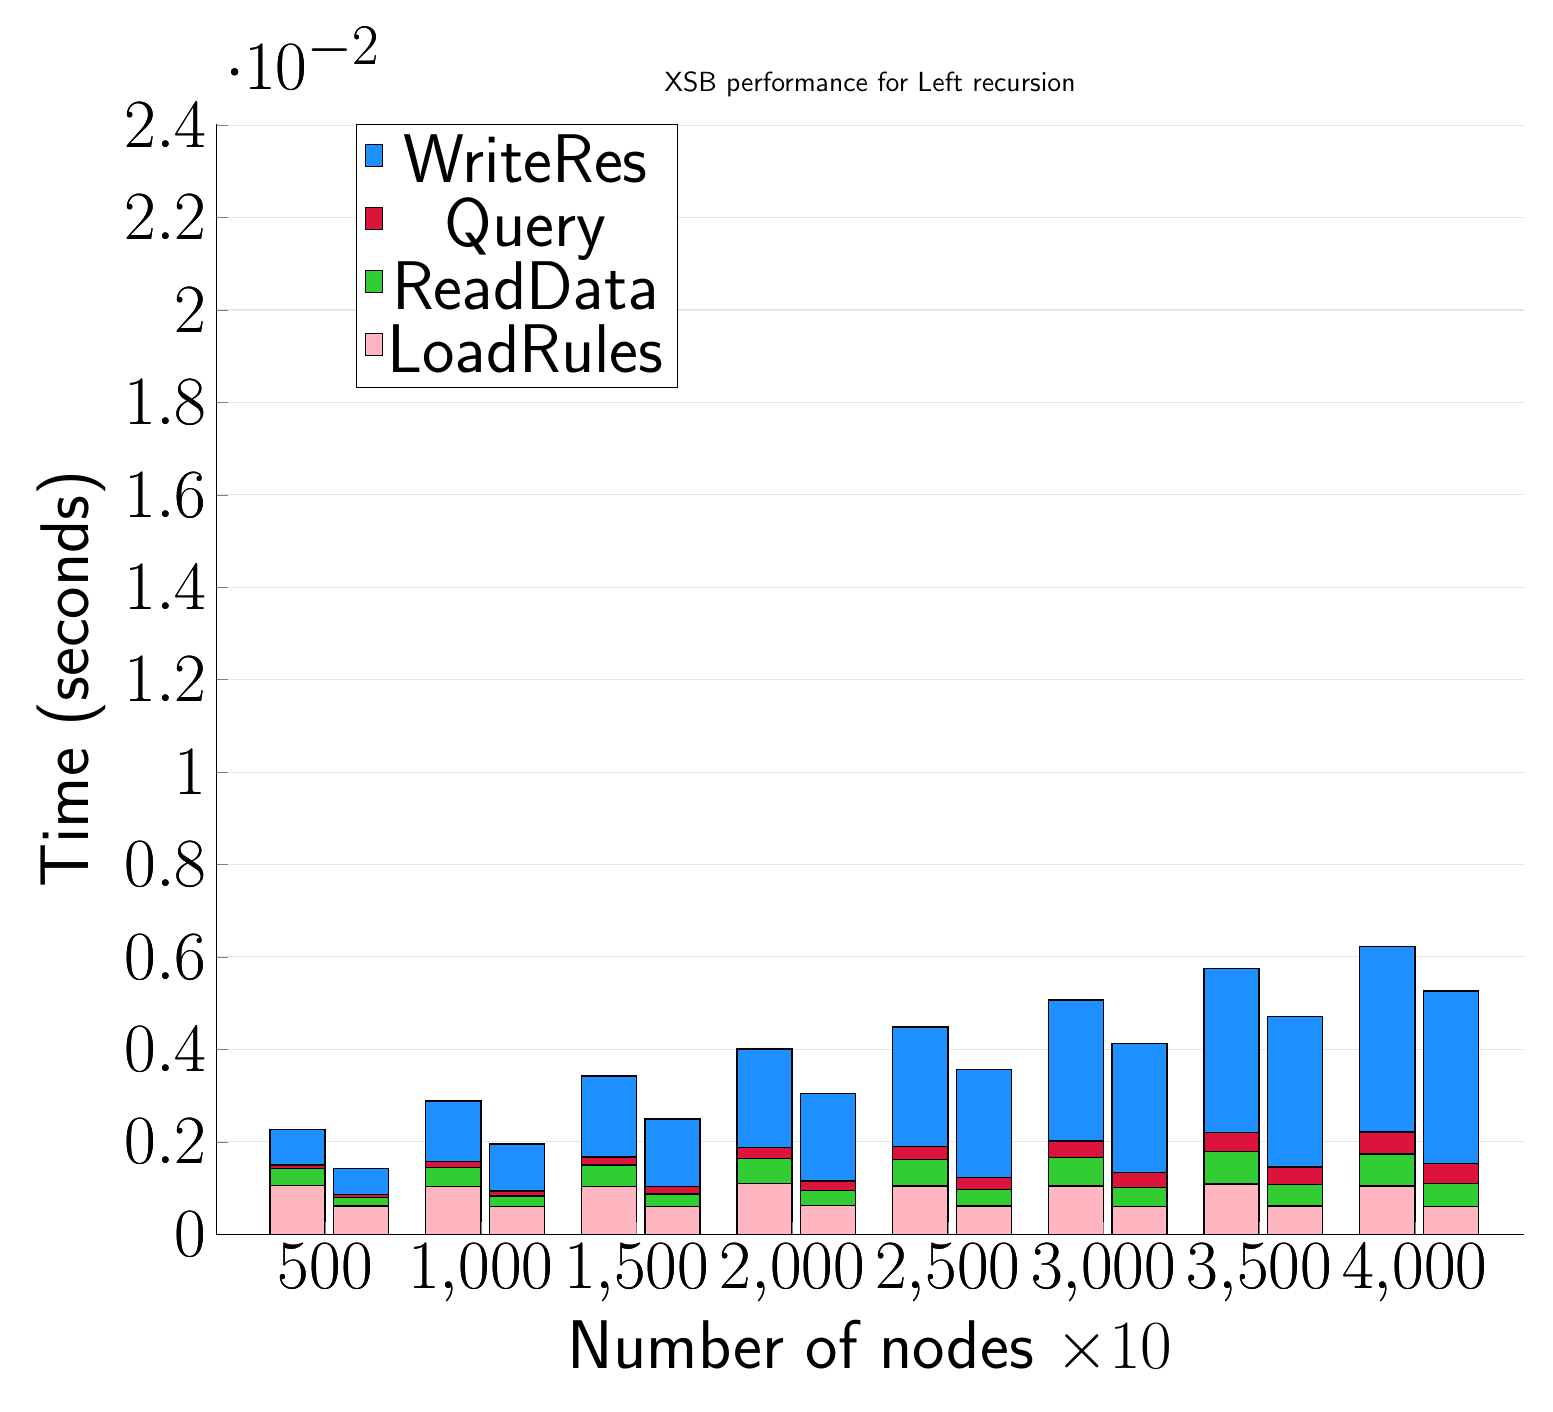
\begin{tikzpicture}
	\begin{axis}[
			ybar stacked,
			title={XSB performance for Left recursion},
			bar shift=-10pt,
			width=1.5\textwidth,
			bar width=0.7cm,
			ymajorgrids, tick align=inside,
			major grid style={draw=gray!20},
			xtick=data,
			ymin=0, ymax=0.024034543037414553,
			axis x line*=bottom,
			axis y line*=left,
			enlarge x limits=0.1,
			legend style={
					at={(0.23, 1)},
					anchor=north,
					legend columns=1,
					font=\Huge,
				},
			ylabel={Time (seconds)},
			xlabel={Number of nodes $\times 10$},
			label style={font=\Huge},
			tick label style={font=\Huge},
		]
		\addlegendimage{fill=DodgerBlue, draw=black, line width=0.2pt}
		\addlegendentry{WriteRes}
		\addlegendimage{fill=Crimson, draw=black, line width=0.2pt}
		\addlegendentry{Query}
		\addlegendimage{fill=LimeGreen, draw=black, line width=0.2pt}
		\addlegendentry{ReadData}
		\addlegendimage{fill=LightPink, draw=black, line width=0.2pt}
		\addlegendentry{LoadRules}
		\addplot +[fill=LightPink, draw=black, line width=0.5pt] coordinates {
				(500, 0.0010606050491333012)
				(1000, 0.001036286354064942)
				(1500, 0.001027917861938476)
				(2000, 0.0011016607284545878)
				(2500, 0.0010451316833496103)
				(3000, 0.0010454177856445309)
				(3500, 0.0010827302932739258)
				(4000, 0.001041412353515626)
			};
		\addplot +[fill=LimeGreen, draw=black, line width=0.5pt] coordinates {
				(500, 0.0003643751144409179)
				(1000, 0.0004132509231567382)
				(1500, 0.0004710674285888672)
				(2000, 0.0005392074584960936)
				(2500, 0.00057222843170166)
				(3000, 0.0006204128265380859)
				(3500, 0.0007100582122802735)
				(4000, 0.000694108009338379)
			};
		\addplot +[fill=Crimson, draw=black, line width=0.5pt] coordinates {
				(500, 7.188320159912111e-05)
				(1000, 0.0001202821731567381)
				(1500, 0.000171995162963867)
				(2000, 0.0002327442169189452)
				(2500, 0.0002761602401733398)
				(3000, 0.0003548622131347655)
				(3500, 0.0004108905792236326)
				(4000, 0.00047249794006347666)
			};
		\addplot +[fill=DodgerBlue, draw=black, line width=0.5pt] coordinates {
				(500, 0.000763416290283203)
				(1000, 0.001310801506042481)
				(1500, 0.00175027847290039)
				(2000, 0.0021362066268920893)
				(2500, 0.002590966224670409)
				(3000, 0.0030471086502075187)
				(3500, 0.0035429000854492196)
				(4000, 0.004022026062011719)
			};
	\end{axis}
	\begin{axis}[
			ybar stacked,
			bar shift=13pt,
			width=1.5\textwidth,
			bar width=0.7cm,
			ymajorgrids, tick align=inside,
			major grid style={draw=none},
			xtick=data,
			ymin=0, ymax=0.024034543037414553,
			axis x line*=none,
			axis y line*=none,
			enlarge x limits=0.1,
			label style={font=\Huge},
			tick label style={font=\Huge},
		]
		\addplot +[fill=LightPink, draw=black, line width=0.5pt] coordinates {
				(500, 0.0006129000000000001)
				(1000, 0.0006027999999999999)
				(1500, 0.0005951000000000001)
				(2000, 0.0006196999999999997)
				(2500, 0.0006086000000000002)
				(3000, 0.0006031999999999997)
				(3500, 0.0006123999999999997)
				(4000, 0.0006034999999999999)
			};
		\addplot +[fill=LimeGreen, draw=black, line width=0.5pt] coordinates {
				(500, 0.0001825999999999997)
				(1000, 0.0002252999999999998)
				(1500, 0.00027229999999999995)
				(2000, 0.0003208000000000003)
				(2500, 0.0003601)
				(3000, 0.0004059000000000004)
				(3500, 0.00046)
				(4000, 0.0004889999999999996)
			};
		\addplot +[fill=Crimson, draw=black, line width=0.5pt] coordinates {
				(500, 6.50000000000005e-05)
				(1000, 0.0001103000000000006)
				(1500, 0.00016129999999999988)
				(2000, 0.00021239999999999947)
				(2500, 0.0002552999999999999)
				(3000, 0.0003301000000000006)
				(3500, 0.00038219999999999997)
				(4000, 0.00043890000000000015)
			};
		\addplot +[fill=DodgerBlue, draw=black, line width=0.5pt] coordinates {
				(500, 0.0005599999999999995)
				(1000, 0.0010156999999999994)
				(1500, 0.0014642000000000001)
				(2000, 0.0018939000000000004)
				(2500, 0.0023398)
				(3000, 0.0027863999999999996)
				(3500, 0.0032530000000000002)
				(4000, 0.0037355)
			};
	\end{axis}
\end{tikzpicture}

\end{document}
